\documentclass[12pt, a4paper]{article}
\usepackage[a4paper, margin=2.5cm]{geometry}
\usepackage[utf8]{inputenc}
\usepackage[swedish]{babel}
\usepackage{amsmath}

\usepackage{graphicx}
\graphicspath{ {images/} }

\usepackage{parskip}
\usepackage{dirtytalk}

\usepackage{fancyhdr}
\pagestyle{fancy}
\fancyhead[L]{\textbf{Namn:} Björn Sundin}
\fancyhead[C]{\textbf{Klass:} TE18C}
\fancyhead[R]{\textbf{Skola:} NTI Kronhus}

\title{Labbrapport: dämpad och driven pendel}
\author{Björn Sundin\medskip\\ TE18C, NTI Kronhus}

\begin{document}

\maketitle

\section{Inledning}
\subsection{Syfte}
\subsection{Frågeställningar}

\subsection{Teori}
Den matematiska modellen som används för att beskriva svängningsrörelsen hos torsionspendeln beskrivs av denna differentialekvation:
\begin{equation}
    \begin{split}
        I\frac{\mathrm{d}^2\theta}{\mathrm{d}t^2}=-k\theta-\lambda\frac{\mathrm{d}\theta}{\mathrm{d}t}+\mu\cos(\omega t)\Leftrightarrow\\
        \theta''(t)+\frac{\lambda}{I}\theta'(t)+\frac{k}{I}\theta(t)=\frac{\mu}{I}\cos(\omega t)        
    \end{split}
\end{equation}
Där: 
\begin{itemize}
    \item $\theta$ är vinkelpositionen av pendeln relativt jämviktsläget i radianer.
    \item $I$ är tröghetsmomentet för pendeln med enhet $[\mathrm{kg}\cdot\mathrm{m}^2$]. Det är vridmomentet som krävs för att skapa en vinkelacceleration på 1 $\frac{\mathrm{rad}}{\mathrm{s}^2}$.
    \item $k$ är vridmomentet per radian vinkelavvikelse riktat mot jämviktsläget för den specifika pendeln. Detta vridmoment orsakar den naturliga svängningen.
    \item $\lambda$ är ett bromsande vridmoment per $\frac{\mathrm{rad}}{\mathrm{s}}$ motriktat rörelseriktningen. Denna orsakar pendelns dämpning.
    \item $\mu$ är amplituden av det pålagda vridmomentet, med frekvensen $\omega [\frac{\mathrm{rad}}{\mathrm{s}}]$.
\end{itemize}
$I$, $k$ och $\lambda$ beror alla på egenskaper hos pendeln samt pendelns radie. $\mu$ beror däremot på den radie där det pålagda vridmomentet appliceras samt kraftens maximum som orsakar vridmomentet.

Differentialekvationen har olika lösningar beroende på värdena på konstanterna:
\begin{enumerate}
    \item Fri pendel: $\lambda=0\land\mu=0\Leftrightarrow\theta(t)=A\sin(\omega_0 t+\phi)$
    \item Dämpad pendel: $\lambda\neq0\land\mu=0\Leftrightarrow\theta(t)=Ae^{-\frac{\lambda}{2}t}\cdot\sin(t\sqrt{\omega_0^2-\frac{\lambda^2}{4}})$
    \item Driven pendel: $\lambda=0\land\mu\neq0\Leftrightarrow\theta(t)=\frac{\mu}{\omega_0^2-\omega^2}\sin(\omega t+\phi)$ där $\omega$ är 
\end{enumerate}
\section{Metod}
\section{Resultat}

Den insamlade datan som mättes med Cassy Lab under laborationen redovisas i figurerna nedan. 

\begin{figure}[hp]
    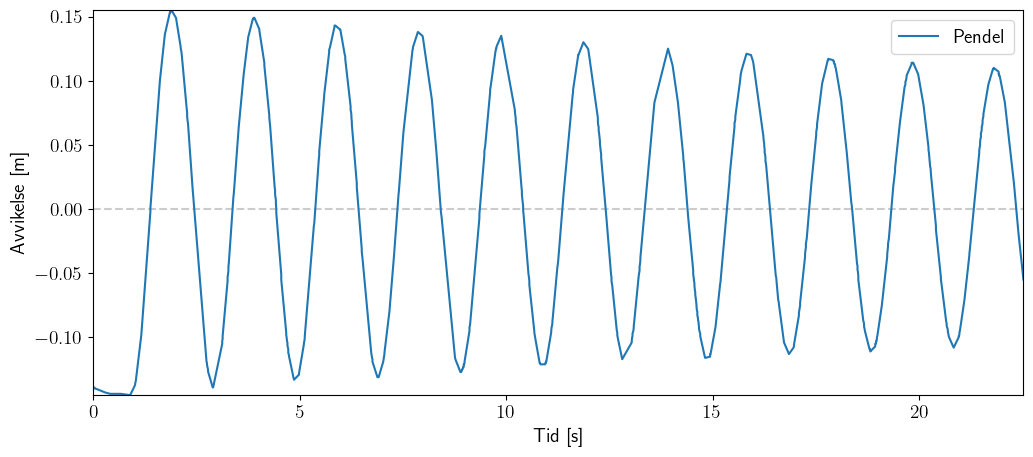
\includegraphics[width=\textwidth]{graf_egenfrekvens}
    \caption{Datan för svängning utan pålagd dämpning.}
\end{figure}

\begin{figure}[hp]
    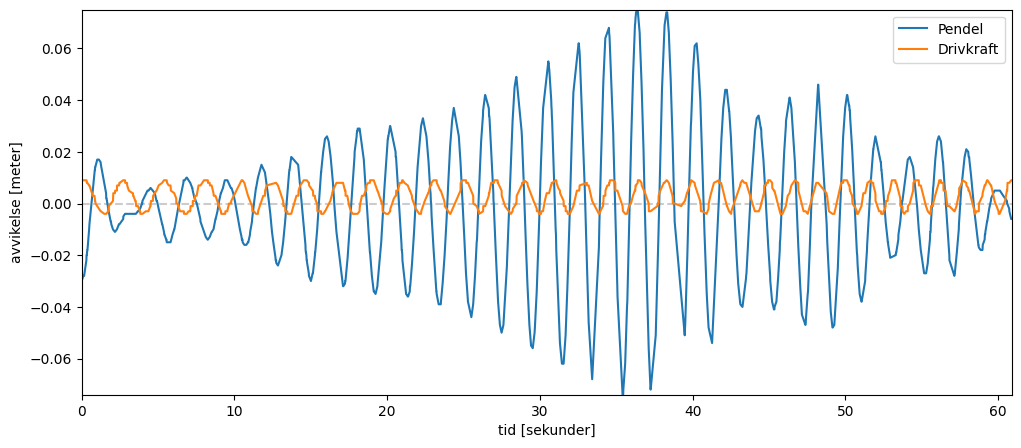
\includegraphics[width=\textwidth]{graf_resonansfrekvens}
    \caption{Datan för driven svängning runt resonansfrekvensen.}
\end{figure}

\section{Analys}

\begin{equation}
    \begin{split}        
        y&=0.1318\cdot\sin((180.63x+103.83)\cdot\frac{\pi}{180})\\
        &\approx0.1318\cdot\sin(3.153x+1.812)    
    \end{split}
\end{equation}
\section{Slutsatser}

\end{document}